\documentclass[12pt]{article}
% We can write notes using the percent symbol!
% The first line above is to announce we are beginning a document, an article in this case, and we want the default font size to be 12pt
\usepackage[utf8]{inputenc}
\usepackage[left=1.2in,top=.8in,right=1.2in,nohead,bottom=.5in]{geometry}
% This is a package to accept utf8 input.  I normally do not use it in my documents, but it was here by default in Overleaf.

\usepackage{amssymb}
\usepackage{amsthm}
\usepackage{commath}
\usepackage{enumerate}
\newtheorem{theorem}{Theorem}
\usepackage{amsmath}
\usepackage{natbib}
\usepackage{thm-restate}
\usepackage{graphicx}
\usepackage{caption}
\usepackage{subcaption}
\graphicspath{ {./plots/} }
\DeclareMathOperator{\Tr}{Tr}
\newcommand{\dd}[1]{\mathrm{d}#1}
\newcommand{\E}{\mathbb{E}}
\newcommand{\Var}{\text{Var}}
\newcommand{\X}{\mathcal{X}}
\newcommand{\B}{\mathcal{B}}
% These three packages are from the American Mathematical Society and includes all of the important symbols and operations 
\usepackage{fullpage}
\usepackage{comment}
% By default, an article has some vary large margins to fit the smaller page format.  This allows us to use more standard margins.

\newcommand{\jx}[1]{{\color{blue}{ #1}}}


\newtheorem{ass}{Assumption}
\newtheorem{lemma}{Lemma}
\newtheorem{corollary}{Corollary}
\setlength{\parskip}{0em}
% This gives us a full line break when we write a new paragraph
\usepackage[mathscr]{euscript}
\usepackage{tikz}
\newcommand*\circled[1]{\tikz[baseline=(char.base)]{
            \node[shape=circle,draw,inner sep=2pt] (char) {#1};}}
\newcommand{\indep}{\perp \!\!\! \perp}
\title{BFGS based quasi-Newton method for acceleration of MM algorithm}
\author{
  Medha Agarwal and Jason Xu
}
\begin{document}

\maketitle

\begin{abstract}
    MM and consequently, EM algorithms are a powerful optimization technique due to both - its simplicity and stability. However, in many statistical applications, they suffer from slow convergence, especially when the dimension of parameter space is high. There has been some work for accelerating the MM algorithm using quasi-Newton methods. These methods attempt to update the approximation for the Jacobian of the algorithm map at each iteration. However, most of them are either too problem-specific or rely on certain conditions on starting values or MM update formula to give acceptable convergence. We propose a quasi-Newton method for accelerating MM algorithms based on the popular BFGS optimization method. However, we are not interested in the optimization problem of the objective function. Our algorithm targets to find the fixed point of the MM algorithm using no specific information about the objective function or its gradient whatsoever. We also propose an LBFGS based algorithm using the same update formulation of Jacobian matrices. The performance of both the algorithms is numerically examined and compared to other quasi-Newton acceleration schemes for MM.
\end{abstract}


\section{Introduction}

MM algorithm is a powerful iterative method for computation of maximum likelihood estimates. It is attractive because of two reasons: (1) MM algorithms are computationally simple to implement and (2) they are stable (monotonous increase in likelihood) (see \cite{dempster1977maximum}; \cite{laird1978nonparametric} and references thereof for discussion on its properties and relevant examples). MM algorithm is much simpler to execute than its alternatives like gradient-based methods (Newton-Raphson) and Fisher score method. A widely discussed drawback with MM algorithms is its slow linear convergence, especially when the amount of missing data is large. (see \cite{wu1983convergence}; \cite{boyles1983convergence}; \cite{meng1994global} for discussion on convergence) and dependence on initial value. 

\jx{I like to give a gentler overview of the motivation and some approaches. The more detailed background with equations etc can be included later in a prior work section. Here is a start:}
To address this shortcoming, there have been a number of works that design acceleration schemes for MM and EM algorithms. Broadly speaking, these methods seek additional information to better inform the search direction and/or step lengths of the unadorned algorithm. Often such information comes from second-order terms, and it is necessary to balance a tradeoff for additional computational cost.
Some approaches directly work with the objective function that the MM algorithm originally seeks to optimize--- in the case of EM, this is the observed data log-likelihood. [Citations to Lange and Jamshidian papers]. Approximate second order information can be obtained via Fisher scoring in the case of EM. Outside of the context of missing data,  classical tools from the numerical optimization literature such as quasi-Newton and conjugate gradient methods can be applied to the objective to similar effect.

These methods may be limited when it is nontrivial to carry out operations such as differentiation with respect to the original objective, and typically rely on handling and storing the approximate Hessian which becomes costly for high-dimensional problems. Indeed, an advantage of MM algorithms lies in sidestepping an intractable objective in favor of operating on surrogates. An alternative approach is to apply acceleration schemes on the sequence of iterates produced by the MM algorithm itself---in other words, to consider acceleration of the MM \textit{algorithm map} instead, largely ignoring the optimization objective. While these often preserve the simplicity and low computational complexity of the original algorithm, they are less firmly rooted in optimization theory. 

[Overview the methods that do so but mention that in many cases they are more ad hoc and do not fully/formally leverage the wisdom in the classical literature and are instead loosely inspired by it.]

\jx{Here I would ``close the introduction" to simply state our contributions and give a very high level description of our proposed approach, contextualizing it in the ``methodological gap" that has been roughly outlined prior. Some things we can highlight is by bridging it to Broyden's method, we get convergence guarantees [hopefully], a way to incorporate additional secant conditions (like Hua's method), efficient low-memory variations, and an explicit decomposition of search direction and step length information. In practice we find that it performs similarly if not better than existing simpler methods in terms of actual runtime, and as suggested by the theory is more robust/reliable across a broad range of settings. Then with that road map in mind the reader can later be exposed to the finer details}.

\jx{What you have written here has lots of good information. Eventually we may split it up so that some references come in the introduction above, some contextualizes relations to existing work after we present our method, and the rest can become part a more specific background/literature review section to follow the introduction}.
There has been wide discussion on methods for accelerating the EM algorithms in statistical community. \cite{varadhan2008simple} suggested a binary classification for EM accelerators - (1) monotone and (2) non-monotone acceleration schemes. Monotone accelerators target to increase the likelihood like EM algorithm. Prominent examples are parameter expansion EM (\cite{liu1998parameter}), Expectation Conditional Maximization (ECM) (\cite{meng1993maximum}), and ECME which shares the monotone convergence properties of EM and ECM while offering a faster convergence (\cite{liu1994ecme}). Non-monotone methods tend to find the root of an objective function, for example, $G(x) = F(x) - x$ where $F(x)$ is the fixed point algorithm map. These methods employ EM iterative schemes to get closer to the root of an objective function which gives the required maximum likelihood estimates. The most widely used and cited method for EM acceleration is the multivariate Aitken's acceleration suggested by \cite{louis1982finding}

\begin{equation}
    \Delta\theta_n = -(J - I)^{-1}g(\theta_n)
\end{equation}

where $\Delta \theta_n$ is the acceleration step, $g(\theta_n)$ is the current step and $J$ denotes the approximation to the Jacobian of the EM step. The method proposed by \cite{louis1982finding} to find $(J - I)$ is essentially the Newton Raphson method to find the zero of $g(x)$ (see discussion by \cite{laird1987maximum}; \cite{meilijson1989fast}). Other examples of monotone accelerators are conjugate gradient (CG) method (\cite{jamshidian1993conjugate}) and quasi Newton methods (\cite{jamshidian1997acceleration}; \cite{lange1995quasi}). The recent acceleration methods STEM and SQUAREM developed by \cite{varadhan2008simple} presents a different category which approximates the Newton's method using the idea of Steffenson's two point secant appoximation for the Jacobian. They build a vector form of this method for STEM and apply an idea of 'squaring' to obtain SQUAREM. \\

The monotone methods are fast and retain the ascent property of EM algorithms. However, they are highly dependent on the intrinsic model properties and hence cannot be broadly applied. Non-monotone methods are generally applicable but lack on the part of storage and globalised convergence. These methods store the Hessian of the algorithm map or require the observed information matrix which limits their use in high dimensional cases. They depend on the starting values and therefore, show poor results when started 'badly'. The SQUAREM requires only the algorithm map for EM and offer great results even for high dimensional problems. Following the work by \cite{varadhan2008simple}, \cite{zhou2011quasi}, built a quasi-Newton acceleration technique that retains the simplicity of SQUAREM. We will call this method ZAL (Zhou Alexander Lange) for future comparisons. As pointed out in \cite{zhou2011quasi}, we are interested in finding the root of the equation $F(x) - x = 0$ unlike the previous quasi Newton methods (\cite{jamshidian1997acceleration}; \cite{lange1995quasi}) that require optimization of the objective function. \\

Both SQUAREM and ZAL do not approximate the full Hessian for optimizing the objective function using Newton's method due to storage and computational complications. ZAL is based on the assumption that we start near the fixed point whereas SQUAREM is based on the assumption that the Jacobian is of the form $\alpha_n I_p$ where $\alpha_n$ is a scalar and $I_p$ is a p-dimensional identity matrix. We propose a quasi Newton acceleration for EM algorithms that instead attempts to approximate the Jacobian of the equation $G(x) = F(x) - x$ for finding its root using Newton's method. The altered approach advocated by ZAL that targets to find the root of $G(x)$ helps us in ignoring the conditions of positive definiteness and makes the algorithm more robust against numerical instabilities. Our method differs from ZAL in the quantity that is minimized given the same constraint. ZAL minimizes the Jacobian of $F(x)$ near the fixed point. This implies that every iterate for Jabobian approximation only depends on the current state and the algorithm map. \\

Our update for the inverse Jacobian approximation takes inspiration from the classical BFGS approach for quasi Newton method. We minimize the spectral norm of the difference between consecutive inverse Jacobian approximations. Our quasi Newton update formula is similar to SQUAREM and ZAL with an added advantage of BFGS robustness for finding the root of $G(x)$. This method surpasses both the assumptions of SQUAREM and ZAL.\\

In high dimensional cases where the number of variables may go up to an order of thousands or millions, the storage costs can be overwhelming. This can limit the application of BFGS algorithms to low dimensional cases only. Limited memory quasi Newton algorithms have been studied by many authors like memory-less quasi-Newton methods (\cite{shanno1978conjugate}) and limited memory BFGS method (\cite{nocedal1980updating}). Another concept of partitioned updating of Hessian matrix by introduced by \cite{griewank1982partitioned}. Limited memory Hessian approximations can also be used as pre-conditioners in conjugate gradient methods (see \cite{buckley1983qn}; \cite{gill2003limited}). Numerical supremacy of L-BFGS has been established by \cite{liu1989limited}. They are simple to implement and do not require an understanding of the structure of Hessian matrix. \\


\section{Quasi-Newton methods for MM acceleration} \label{sec:qn}

Building on work established by \cite{varadhan2008simple} and \cite{zhou2011quasi}, we will use a Newton-type method to accelerate the convergence of an MM algorithm map to its fixed point. The popular BFGS update formula is a quasi-newton method that works towards optimizing a function by approximating its Hessian at each step. Consider the MM algorithm map $F: \mathbb{R}^p \to \mathbb{R}^p$. Instead of solving the parent optimization problem, we are interested in finding the roots of the objective function $G(x) = F(x) - x$. This altered approach of finding the root of $G(x)$ using quasi-Newton method requires one to only update the Jacobian approximation of $G(x)$ at each step instead of a Hessian matrix.

The Steffenson type EM (STEM) method suggested by \cite{varadhan2008simple} achieves this approximation using a scalar multiple of identity matrix. This scalar can be understood as the steplength for each update. The same steplength is used to arrive at the SQUAREM method. While SQUAREM outperforms many acceleration methods and is chiefly regarded for its simplicity, the loss of information due to approximation of Jacobian by an identity matrix can be severe, especially in high dimensional cases. We propose approximating the full Jacobian matrix at each iterate.

However, storage and calculation of the full $p \times p$ dimensional Jacobian at each iteration can be a computationally challenging task which will limit its application for a high-dimensional problem. To surpass this limitation, we will also present an L-BFGS based quasi-newton algorithm which does not require to store the full dense $p \times p$ inverse Jacobian matrix. Instead, one is only required to store some pre-specified $m$ numbers of iterations to approximate the inverse Jacobian. In the next two subsections, we present both the algorithms and their theoretical comparison to other quasi-Newton algorithms like SQUAREM and ZAL. 

\subsection{BFGS based quasi-Newton method}
Our method begins with a simple core idea: first, denote the algorithm map $F$, i.e.  $F: x_k \mapsto x_{k+1}$ where $x_k$ is the $k$th iterate of the unaccelerated MM algorithm. An MM algorithm seeks to optimize some objective function, but can equivalently be expressed without reference to that objective as seeking the fixed points of the algorithm map. That is, we seek roots of the equation $G(x) = F(x) - x$. The observation allows us to employ quasi-Newton acceleration to $G$. The iterative update formulation using Newton's method is given by:
\[
    x^{n+1} = x^n - (dF(x^n) - I)^{-1}G(x^n)    
\]

Let $H^n$ be an approximation of $(dF(x^n) - I)^{-1}$, then the quasi-Newton update formula is given by
\[
x^{n+1} = x^n - H^n G(x^n)\,.
\]
The secant approximation required for quasi Newton method can be obtained by using two consecutive updates from the algorithm map starting from the current position. We will follow the same secant approximation recommended by \cite{zhou2011quasi}, where the function $G(x)$ us assumed to be linear between $x_t$ and $F(x_t)$ with the inverse Jacobian given by $H_{t+1}$

\begin{equation} \label{eq: secant_approx}
    H^{t+1}\left[G(F(x_t)) - G(x_t)\right] = F(x_t) - x_t.    
\end{equation}


Let us define $v_t = G(F(x_t)) - G(x_t) = F^2(x_t) - 2F(x_t) + x_t$ and $u_t = F(x_t) - x_t$, then the secant requirement is $H^{t+1}v_t = u_t$. \jx{I edited this section, but here we might add a clearer transition to emphasize the fact that one needs to specify additional information in order for the solution to be well-defined rather than underdetermined, and in particular we will instead make use of the objective that allows us to recover Broyden's method for accelerated nonlinear root-finding}. 

We propose a quasi Newton update which optimizes the next iterate of Jacobian, such that $\|H_{t+1}-H_t\|_F$ is minimum and also, the secant approximation constraint is met. In fact, for the best results we require several secant approximations $H_t (u_t^i - v_t^i) = u_t^i$ for $i \in \{1, ..., q\}$. These can be generated at the current iterate $x^t$ and previous $(q-1)$ iterates. Let $U_t = (u_1\;u_2 \dots u_q)$ and likewise $V_t = (v_1 \; v_2 \dots v_q)$ be two $\ \times q$ matrices. The optimization problem becomes,

\begin{center}
    Minimize: $\|H_{t+1} - H_t\|_F$\\
    Constraint: $H_{t+1}V_t = U_t\;$ .
\end{center}

We take the partial derivative of the Lagrangian
\[
\mathcal{L} = \dfrac{1}{2}\|H_{t+1} - H_t\|^2_F + \Lambda^T(H_{t+1}V_t - U_t)
\]
with respect to $h_{t+1}^{ij}$ and equate to 0. Here $h_{t+1}^{ij}$ denotes the $ij^{th}$ element of the matrix $H_{t+1}$. As a consequence, we get the Lagrange multiplier equation:
\[
0 = h_{t+1}^{ij} - h_t^{ij} + \sum_{k=1}^{p}\lambda_{ik}v_{jk}
\]
In matrix notation, we have,
\begin{equation} \label{eq:legrange_eq1}
H_{t+1} - H_t + \Lambda V_t^T = 0    
\end{equation}
Post multiply equation~\ref{eq:legrange_eq1} by $V_t$ and put $H_{t+1}V_t = U_t$

\begin{align*}
    H_{t+1}V_t - H_tV_t + \Lambda V_t^T V_t &= 0
\end{align*}
This implies
\[
     \Lambda = (H_t V_t - U_t)(V_t^TV_t)^{-1}\,.
\]
Therefore, 
\[
H_{t+1} = H_t\left(I - V_t (V_t^T V_t)^{-1}V_t^T\right) + U_t(V_t^T V_t)^{-1}V_t^T.
\]

Although as the problem dimension increases, higher $q$ should give tigher convergence to the fixed point, however numerically we might face singularity for the matrix $V_t^T V_t$. The special case of $q=1$ is the most successful  where:
\begin{equation} \label{eq:BFGS_update}
    H_{t+1} = H_t - H_t\dfrac{v_tv_t^T}{v_t^Tv_t} + \dfrac{u_tv_t^T}{v_t^Tv_t}\,.
\end{equation}

Equation \ref{eq:BFGS_update} can be written as $H_{t+1} = H_t + A_t + B_t$ where both $A_t$ and $B_t$ are rank-1 matrices. Therefore, as expected Equation~\ref{eq:BFGS_update} is a rank-2 update. The symmetry condition on $H_t$ assumed in classical BFGS update can be dropped here because it approximates a Jacobian matrix instead of a Hessian matrix.

\paragraph{Intuition and relation to prior work} 
 The search direction at $t^{th}$ iteration is given by $p_t = -H_{t}G(x_t)$ and the update formula is 
\[
x_{t+1} = x_t + \gamma_t p_t
\]
where $\gamma_t = \alpha_t /\|p_t\|$ is an appropriate scaling factor in the search direction and $\alpha_t$ is the steplength. Notice that the steplength for non-accelerated MM algorithm is $\|F(x_t) - x_t\| = \|u_t\|$. Suppose we use the steplength $\|H_t\| \|G(x_t)\|$ in the search direction $p_t = -H_tG(x_t)$. If $H_t$ is sufficiently close to $H_{t+1}$, using Equation~\ref{eq: secant_approx} we can lowebound $\|H_t\|$ by $\|u_t\|/\|v_t\|$. We will use this lowerbound of steplength giving $\alpha_t = \|u_t\|^2/\|v_t\|$. The SQUAREM algorithm provides three different possible steplengths along the direction $u_t$. Notice that our choice of $\alpha_t$ coincides with the third steplength. Likewise, we can construct $\alpha_t$ corresponding to the first and second steplengths of SQUAREM. In this paper, we will only focus on the $\alpha_t$ explicitly mentioned above.
\jx{We can further flesh out this subsection, and emphasize exactly why this is more general than the SQUAREM methods and how it sort of unifies existing methods, and also why it is potentially a better formulation than ZAL. We should close this with a discussion on the drawback that our formulation, while closer to established wisdom, leads to a Jacobian that can be unwieldy, and the design of ZAL is more immediately applicable to high-dimensional problems. This then transitions into the next section}


\subsection{L-BFGS based quasi-Newton method}


Our algorithm requires storage of $H_{t}$ before performing a rank-two update on it by Equation~\ref{eq:BFGS_update}. The cost of storing the $n \times n$ inverse Hessian matrix for each update can limit the application of this method for high dimensional problems. Many limited memory quasi-Newton algorithms have been proposed (see \cite{shanno1978conjugate}; \cite{nocedal1980updating}; \cite{griewank1982partitioned}). Here we will focus on L-BFGS method by extending our BFGS based quasi-Newton accelerator to the L-BFGS analogue using the same Jacobian update formulation. Recall that $H_{t}$ is updated by the formula
\[
    H_{t+1} = H_{t}\left(I - \dfrac{v_t v_t^T}{v_t^T v_t}\right) + \dfrac{u_t v_t^T}{v_t^T v_t} = H_t W_t +.\dfrac{u_t v_t^T}{v_t^T v_t}
\]
where $W_t = \left( I- v_t v_t^T/v_t^T v_t\right)$ and the BFGS update is given by $x_{t+1} = x_t - H_t(F(x_t) - x_t)$. Similar to the L-BFGS method, we will store previous $m$ (usually between 3 to 20) pairs of $\{u_i, v_i\}$, $i = t-1, ..., t-m$. The product responsible for update at each step, i.e. $H_t G(x_t)$ is obtained by performing a sequence of inner products and vector summations involving $G(x_t)$ and the pairs $\{u_i, v_i\}$. After the new iterate is computed, the oldest vector pair $\{u_{(t-m)}, v_{(t-m)}\}$ is replaced by the new pair $\{u_{t+1}, v_{t+1}\}$ obtained from the current step. In this way, the set of vector pairs includes curvature information from the $m$ most recent iterations.

An initial estimate of inverse Hessian at $t^{th}$ step is considered to be a scalar multiple of identity matrix. Let us denote this by $H_t^0$. This initial approximation can vary from iteration to iteration, unlike standard BFGS method. Following this $H_t^0$ is updated $m$ times via Equation \ref{eq:BFGS_update} in a nested manner to obtain the following relation

\begin{align*}
    H_{t} &= H_t^0 (W_{t-m} ... W_{t-1})\\
            &+ \dfrac{u_{t-m} v_{t-m}^T}{v_{t-m}^T v_{t-m}}(W_{t-m+1}...W_{t-1})\\
            &+ \dfrac{u_{t-m+1} v_{t-m+1}^T}{v_{t-m+1}^T v_{t-m+1}} (W_{t-m+2}...W_{t-1})\\
            &+ ...\\
            &+ \dfrac{u_{t-1} v_{t-1}^T}{v_{t-1}^T v_{t-1}}\,.
\end{align*}

Let $H_t^0$ be written as $\nu_tI$ where $\nu_t$ is a scalar that varies from iteration to iteration. Chapter 6 from \citet{nocedal2006numerical} explain the effectiveness of using

\[
 \nu_t = \dfrac{u_{t}^T v_{t}}{v_{t}^T v_{t}}.
\]
\\
As discussed there, $\nu_t$ is the scaling factor that attempts to estimate the size of the true Hessian matrix along the most recent search direction. One can observe that STEM method of EM acceleration by \cite{varadhan2008simple} is similar L-BFGS method described above in the sense that it corresponds to L-BFGS with $m=0$. However it is worth to note that they arrived at the approximation of inverse Hessian matrix as $\nu_t I$ by minimizing the distance between the zeros of two linear secant-like approximations for $G(x)$; one centered around $x_t$ and another at $F(x_t)$.

\subsection{Properties}
\jx{Add remark that this respects/preserves any linear constraints that may have originally been enforced. Add convergence results or highlight existing theorems that can apply under appropriate assumptions}

\section{Examples and Performance} \label{subsec:BFGSex}

We will compare five methods for the examples below: (1) non-accelerated MM method, (2)ZAL for $q = 2$, (3) SQUAREM (all three variates) (4) BFGS based QN method, and (5) L-BFGS based QN method. Both ZAL and SQUAREM offer scalar approximations for the Jacobian method. As a consequence, they are pretty fast to implement. For a high-dimensional problem, BFGS based QN method offer extremely slow convergence. However, we are interested in ascertaining the fast convergence of BFGS method for a moderately dimensional problem, and study the performance of L-BFGS as compared to BFGS method for high dimensional cases. We observe striking results for our algorithms in most of the examples. At other times, they perform as good as the other aforementioned acceleration algorithms. The termination criterion for each example is to stop at $x^*$ such that $\|F(x^*) - x^*\| \leq \epsilon$ where $\epsilon$ is fixed at $10^{-7}$ for each example. 

\subsubsection{Truncated Beta Binomial} \label{ex:trunc.beta.binom}

\begin{table}[h]
\centering
\begin{tabular}{c c c c c c c} 
 \hline
 Household & \multicolumn{4}{c}{Number of cases} & \multicolumn{2}{c}{MLE} \\ [0.5ex] 
     & 1 & 2 & 3 & 4 & $\hat{\pi}$ & $\hat{\alpha}$ \\ [0.5ex]
 \hline
 (a) & 15 & 5 & 2 & 2 &  0.0000 & 0.6151 \\ 
 (b) & 12 & 6 & 7 & 6 & 0.1479 & 1.1593 \\
 (c) & 10 & 9 & 2 & 7 & 0.0000 & 1.6499 \\
 (d) & 26 & 15 & 3 & 9& 0.0001 & 1.0594 \\[1ex] 
 \hline
\end{tabular}
\caption{The Lidwell and Somerville (1951) cold data on households
of size 4 and corresponding MLEs under the truncated beta-binomial
model}
\label{tab:bet_binom_data}
\end{table}
We consider the cold incidence dataset by \cite{lidwell1951observations} and fit a zero-truncated beta binomial model because the households reported have at least one cold incidence. Table~\ref{tab:bet_binom_data} summarizes the dataset where the households were classified as: (a) adults only; (b) adults and school children; (c) adults and infants; and (d) adults,
school children, and infants. Suppose $n$ is the total number of independent observations (households) and $x_i$ denotes the number of cold cases in the $i^{th}$ household. This is a discrete probability model with likelihood given by
\[
L(\theta | X) = \prod_{i=1}^{n}\dfrac{g(x_i| \theta)}{1-g(0|\theta)}\,.
\]
Here $g(x|\theta)$ is the probability density function for a beta binomial distribution with parameter vector $\theta$ and maximum count of $m=4$. Here $\theta = (\alpha, \pi)$ such that $\pi \in (0,1)$ and $\alpha >0$. The MM algorithm updates are given by 

\begin{align*}
    \alpha_{t+1} &= \dfrac{\sum_{k=0}^{m-1} (\dfrac{s_{1k}k \alpha_t}{\pi_t + k\alpha_t} + \dfrac{s_{2k}k \alpha_t}{1 - \pi_t + k\alpha_t})}{\sum_{k=0}^{m-1}\dfrac{r_k k }{1 + k \alpha_t}}\\
    \pi_{t+1} &= \dfrac{\sum_{k=0}^{m-1}\dfrac{s_{1k}\pi_t}{\pi_t + k\alpha_t}}{\sum_{k=0}^{m-1}(\dfrac{s_{1k \pi_t}}{\pi_t + k \alpha_t} + \dfrac{s_{2k}(1-\pi_t)}{1- \pi_t + k \alpha_t})}
\end{align*}
where $s_{1k}, \, s_{2k},\, r_k$ are pseudo counts given by
\begin{align*}
    s_{1k} &= \sum_{i=1}^{n}1_{x_i \geq k+1}\\
    s_{2k} &= \sum_{i=1}^{n} \left[ 1_{x_i \leq m-k-1} + \dfrac{g(0|\pi_t, \alpha_t)}{1 - g(0 | \pi_t, \alpha_t)} \right]\\
    r_k &= \sum_{i=1}^{n}\left[ 1 +  \dfrac{g(0|\pi_t, \alpha_t)}{1 - g(0 | \pi_t, \alpha_t)} \right] 1_{t \geq k+1}\,.
\end{align*}



\begin{table}[h!]
\centering
\begin{tabular}{c | c c c c c} 
 \hline
 Data & Algorithm & -ln L & Fevals & Iterations & Time \\ [0.5ex] 
 \hline
 (a) & MM & 25.2282 & 17898 & 17989 & 2.647 \\ 
   & BFGS, $q=1$ & 25.2287 & 26 & 14 & 0.043 \\
   & BFGS, $q=2$ & 25.2276 & 29 & 16 & 0.039\\
   & SqS1 & 25.2282 & 1343 & 661 & 0.208\\
   & SqS2 & 25.2280 & 51 & 18 & 0.0279\\
   & SqS3 & 25.2282 & 54 & 19 & 0.0289\\
   & ZAL, $q=1$ & 25.2270 & 66 & 33 & 0.035\\[1ex]
 (b) & MM & 41.7286 & 5492 & 5492 & 0.748 \\
   & BFGS, $q=1$ & 41.7286 & 928 & 470 & 0.270\\
   & BFGS, $q=2$ & 41.7286 & 1107 & 555 & 0.316\\
   & SqS1 & 41.7286 & 254 & 115 & 0.039\\
   & SqS3 & 41.7286 & 99 & 34 & 0.027\\
   & ZAL, $q=1$ & 41.7286 & 524 & 262 & 0.105\\
   & ZAL, $q=2$ & 41.7286 & 593 & 297 & 0.141\\ [1ex]
  (c) & MM & 37.358 & 61843 &  61843 & 5.891\\
  & BFGS, $q=1$ & 37.358 & 1870 & 936 & 0.624\\
   & BFGS, $q=2$ & 37.358 & 63 & 33 & 0.061\\
   & SqS1 & 37.358 & 2799 & 1388 & 0.406 \\
   & SqS3 & 37.358 & 120 & 41 & 0.035 \\
   & ZAL, $q=1$ & 37.358 & 1292 & 646 & 0.495\\
   & ZAL, $q=2$ & 37.358 & 60 & 32 & 0.036 \\[1ex]
  (d) & MM & 65.042 & 25026 & 25026 & 2.797 \\
   & BFGS, $q=1$ & 65.043 & 268 & 135 & 0.117 \\
   & BFGS, $q=2$ & 65.041 & 57 & 30 &  0.087 \\
   & SqS1 & 65.041 & 1197 & 587 & 0.200 \\
   & SqS3 & 65.042 & 60 & 21 & 0.029 \\
   & ZAL, $q=2$ & 65.040 & 49 & 25 & 0.031 \\ [1ex]
 \hline
\end{tabular}
\caption{Comparison of algorithms for the Lidwell and Somerville
Data. The starting point is $(\pi,\alpha) = (0.5, 1)$, the stopping criterion
is $\epsilon = 10^{-7}$, and the number of parameters is two.}
\label{tab:beta_binom}
\end{table}

\begin{figure}
    \centering
    \begin{subfigure}[h]{0.45\textwidth}
        \centering
        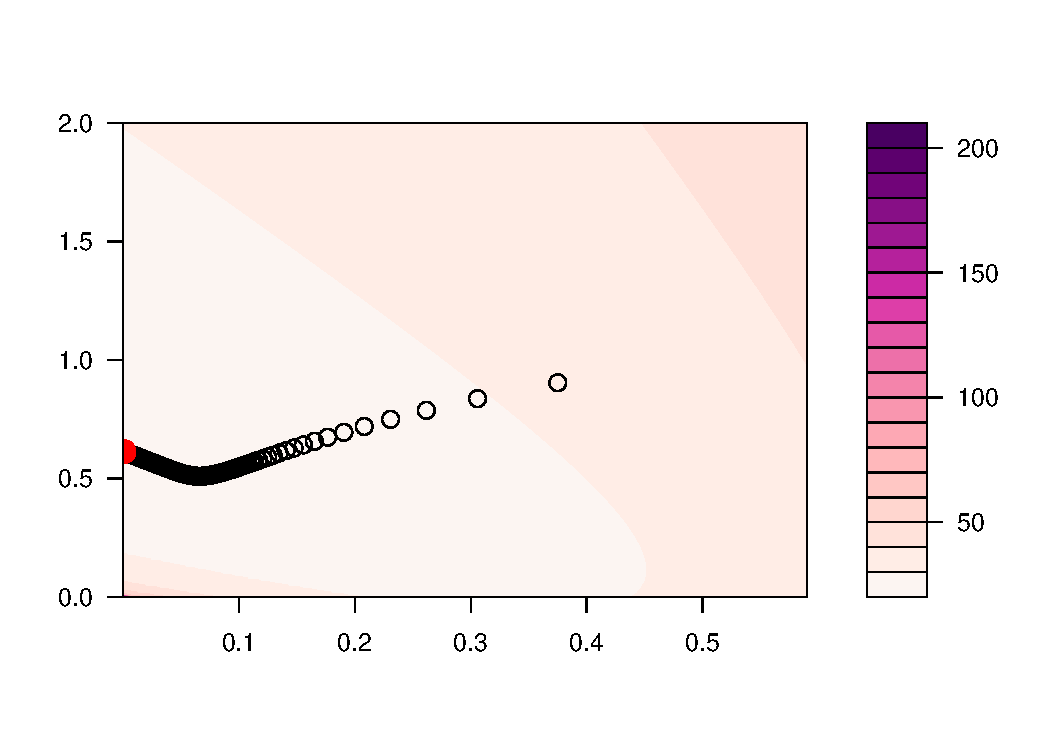
\includegraphics[width = \textwidth]{plots/beta-contour_MM.pdf}
        \caption{MM}
        \label{}
    \end{subfigure}
    \begin{subfigure}[h]{0.45\textwidth}
        \centering
        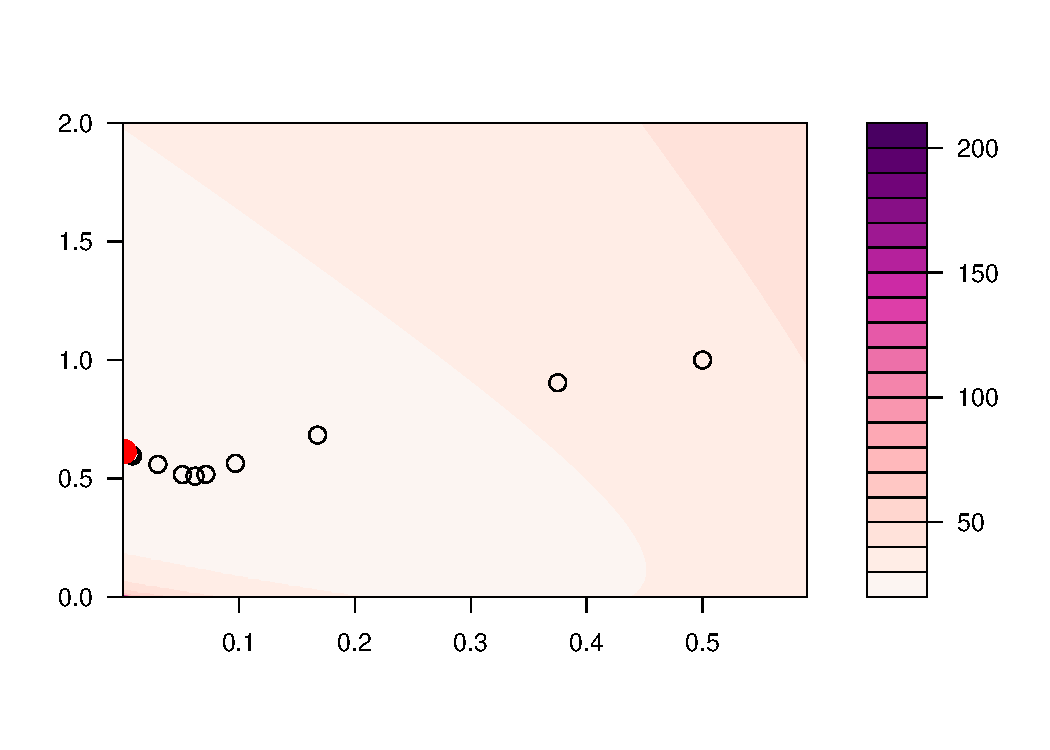
\includegraphics[width = \textwidth]{plots/beta-contour_BFGS1.pdf}
        \caption{BFGS, $q=1$}
        \label{}
    \end{subfigure}\\
    \begin{subfigure}[h]{0.45\textwidth}
        \centering
        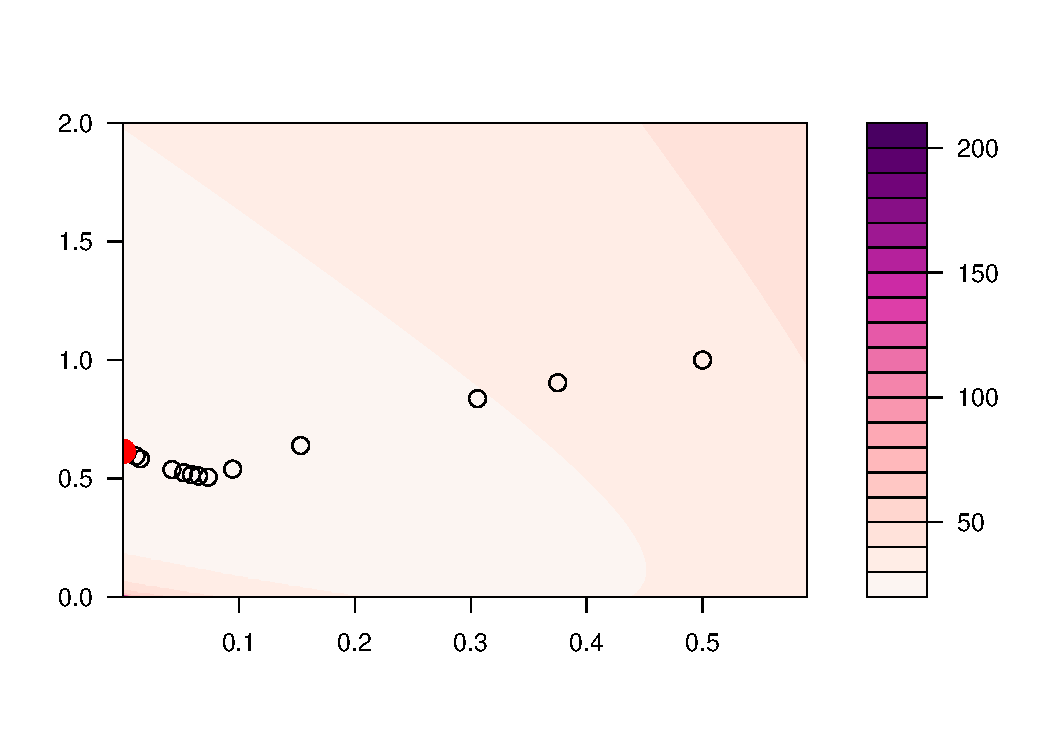
\includegraphics[width = \textwidth]{plots/beta-contour_BFGS2.pdf}
        \caption{BFGS, $q=2$}
        \label{}
    \end{subfigure}
    \begin{subfigure}[h]{0.45\textwidth}
        \centering
        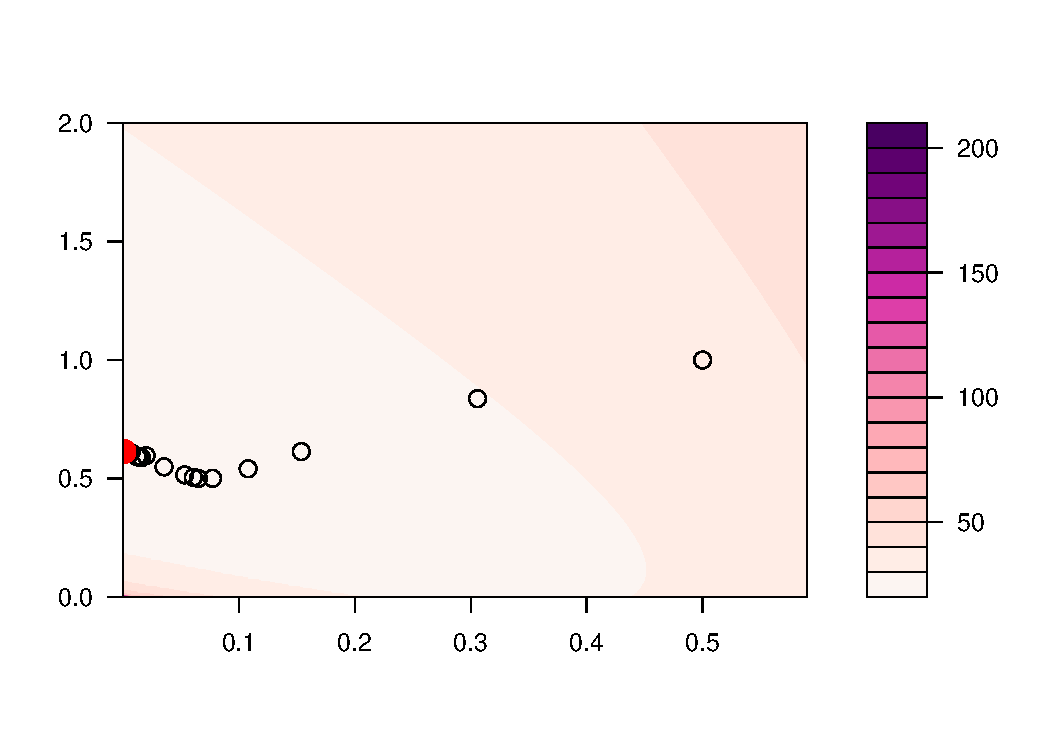
\includegraphics[width = \textwidth]{plots/beta-contour_SqS1.pdf}
        \caption{SqS1}
        \label{}
    \end{subfigure}\\
    \begin{subfigure}[h]{0.45\textwidth}
        \centering
        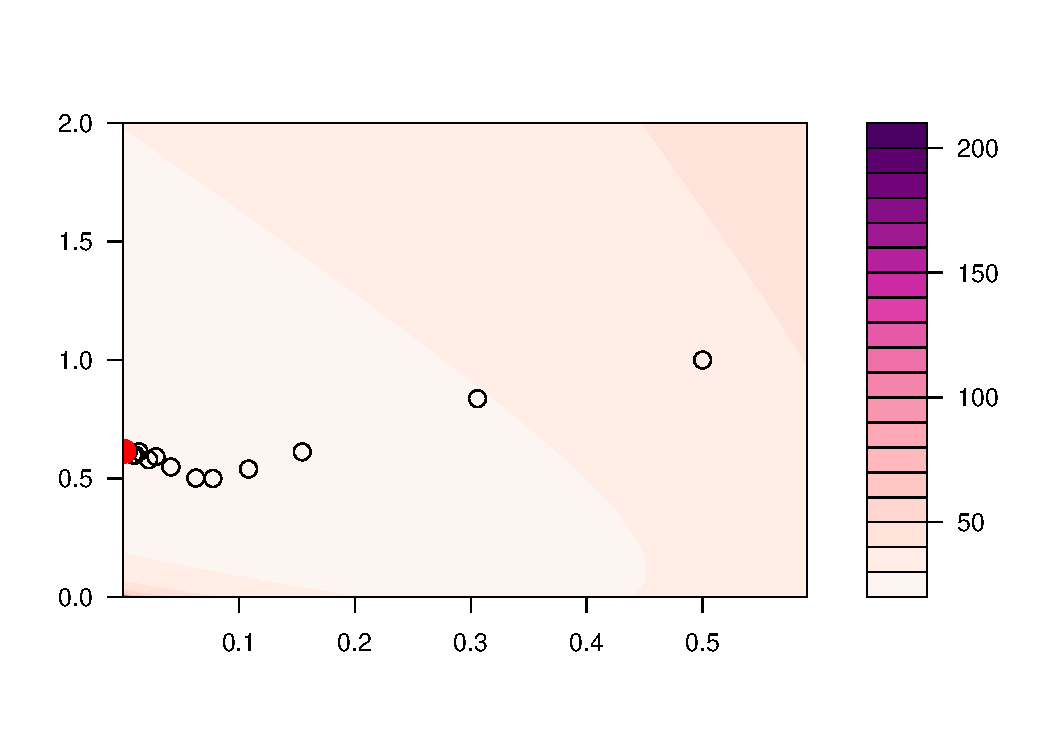
\includegraphics[width = \textwidth]{plots/beta-contour_SqS2.pdf}
        \caption{SqS3}
        \label{}
    \end{subfigure}
    \begin{subfigure}[h]{0.45\textwidth}
        \centering
        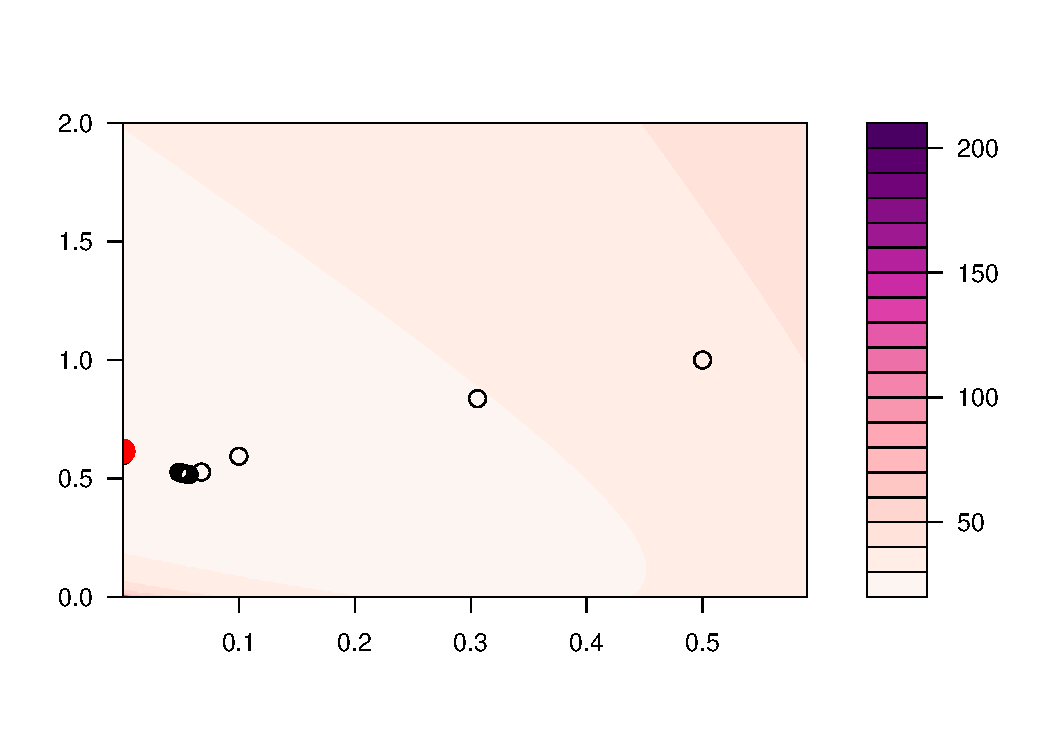
\includegraphics[width = \textwidth]{plots/beta-contour_ZAL1.pdf}
        \caption{ZAL, $q=1$}
        \label{}
    \end{subfigure}\\
    \caption{Truncated Beta Binomial. Ascent of different methods for Somerville household type (a) data. Starting points are $(\pi_0, \alpha_0) = (0.5, 1)$. The tolerance is $\epsilon = 10^{-7}$.}
    \label{fig:beta-contour}
\end{figure}

Table \ref{tab:beta_binom} lists the final negative log-likelihood, number of MM evaluations, number of algorithm iterations, and running times until convergence for each algorithm is achieved for all the four cases. The starting point is $(\pi,\alpha) = (0.5, 1)$. In the last three cases, SQUAREM-2 fails to converge to the truth. It can be observed that BFGS with $q=2$ provides significant improvement over $q=1$ case for the third and fourth case. Except for second case, BFGS with $q=2$ either outperforms or performs at least as good as other acceleration schemes. Figure~\ref{fig:beta-contour} shows the progress path of all the algorithms on a contour plot for the first data type. Notice that in this case, our algorithm provides the fastest convergence.



\subsubsection{Generalized eigenvalues} \label{ex:gen.eigen}
\begin{table}[!htbp]
\centering
\begin{tabular}{c c c c c} 
 \hline
 Algorithm & \multicolumn{2}{c}{Largest Eigenvalue} & \multicolumn{2}{c}{Smallest Eigenvalue} \\ [0.5ex] 
 & Evals & Time & Evals & Time\\ [0.5ex]
 \hline
MM  & 29654 & 13.9217 & 33822 & 23.2785\\ 
BFGS & 1966 & 2.6628 & 3016 & 4.7921 \\
LBFGS & 2022 & 2.1103 & 2557 &  2.9211 \\
SqS1 & 2571 & 1.3733 & 1971 & 1.7423 \\
SqS2 & 2571 & 1.5673 & 1971 & 1.9398 \\
SqS3 & 2571 & 1.3833 & 1971 & 1.6266 \\
ZAL & 19077 & 13.7742 & 23875 & 17.7076\\ [1ex] 
 \hline
\end{tabular}
\caption{Generalized eigenvalues. Number of $F(x)$ evaluations and running times random matrices A and B of dimension $100 \times 100$. Here the stopping criterion is $\epsilon = 10^{-7}$, and the number of parameters
is 100. The starting vector is randomly chosen.}
\label{tab:gen_eigen}
\end{table}
Because of the zigzag nature of steepest ascent, naive acceleration performs poorly. If $x_{n+1} = F(x_n)$ is the algorithm
map, the Naive and Zhou's method is calculated using $F_s(x)$ as the algorithm map which is its s-fold functional composition. This substitution preserves the ascent property. Table \ref{tab:gen_eigen} shows the
results of accelerating two-step (s = 2) steepest ascent and
steepest descent. \\


\begin{figure}
    \centering
    \begin{subfigure}[!htbp]{0.45\textwidth}
        \centering
        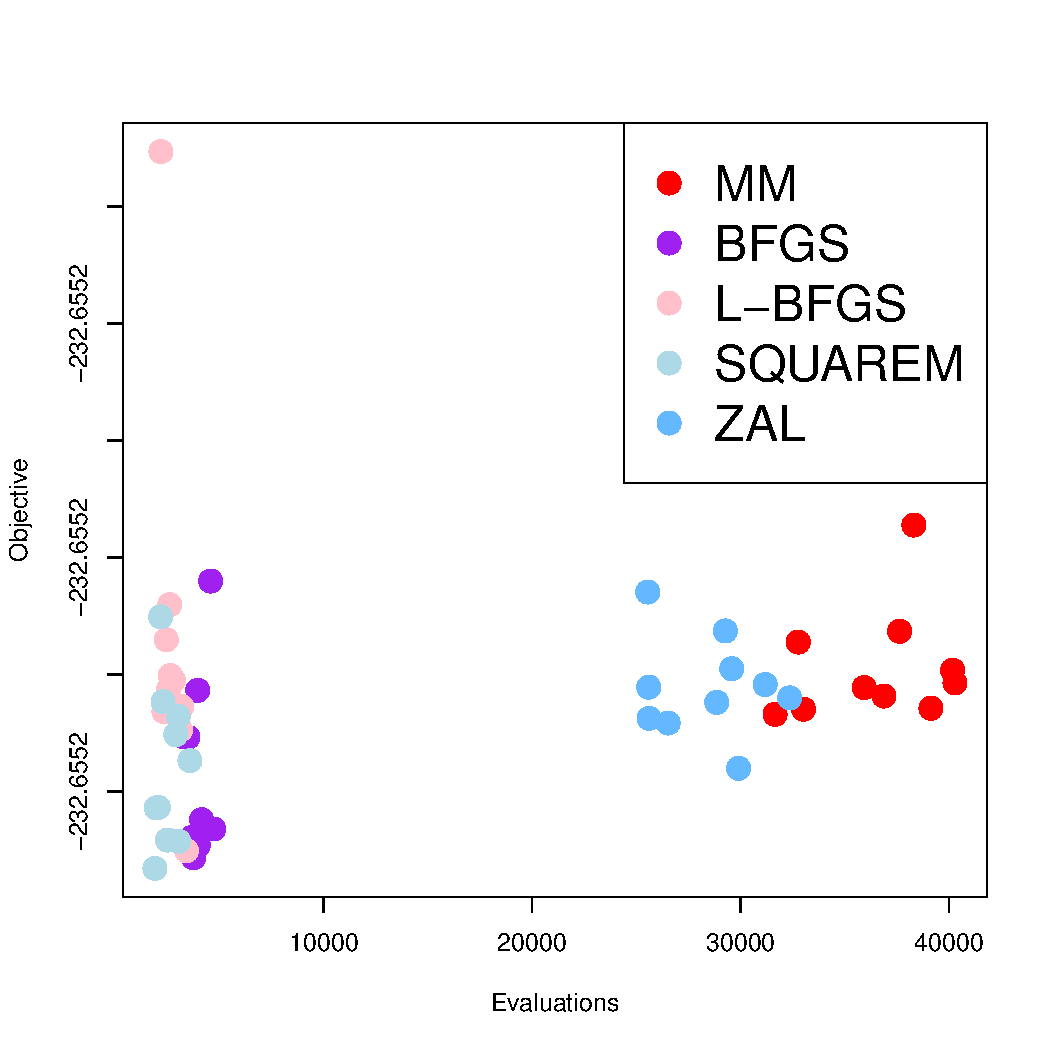
\includegraphics[width = \textwidth]{plots/eigen-objVSeval_sd10.pdf}
        \caption{Objective vs Number of F evaluations}
        \label{subfig:eigen-objVSeval}
    \end{subfigure}
    \begin{subfigure}[h]{0.45\textwidth}
        \centering
        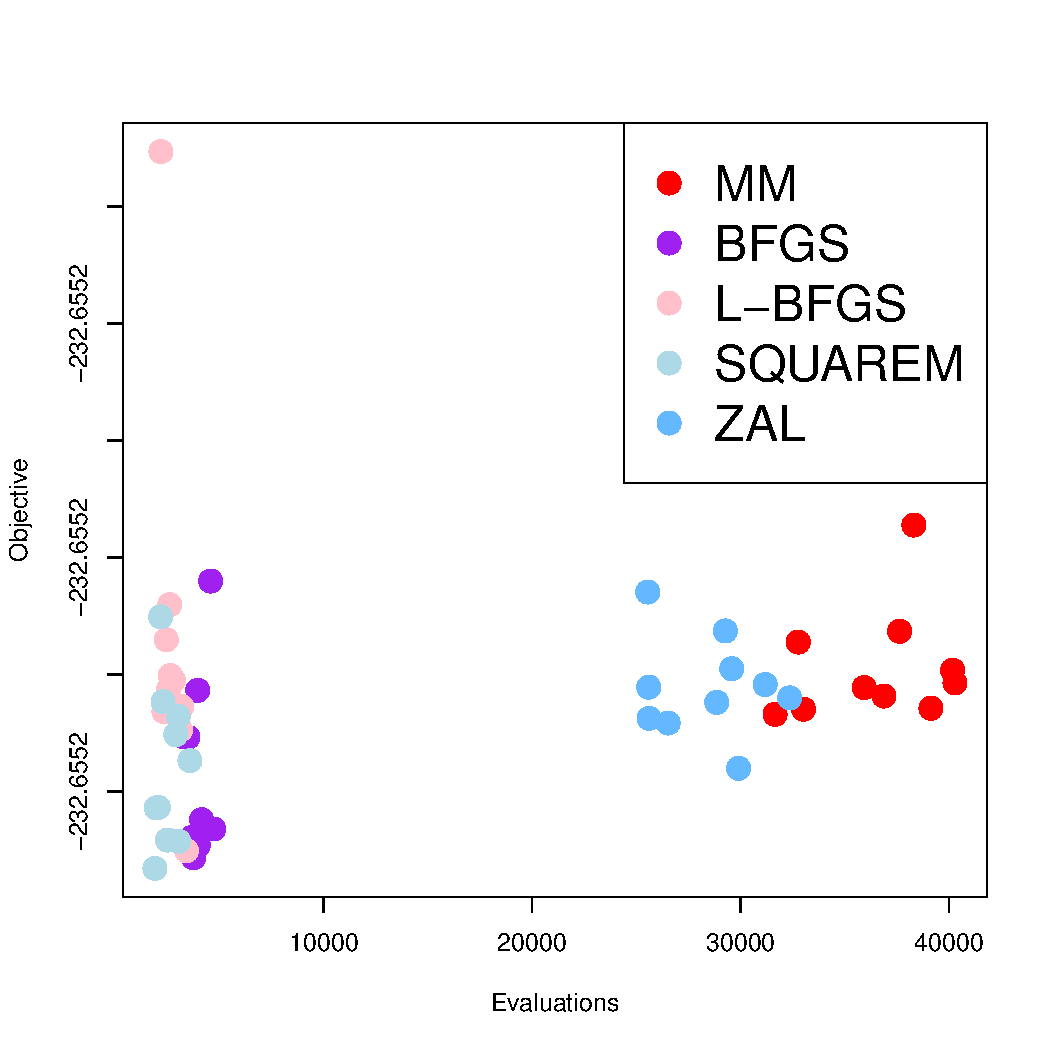
\includegraphics[width = \textwidth]{plots/eigen-objVSeval_sd10.pdf}
        \caption{Objective vs Time}
        \label{subfig:eigen-objVSeval}
    \end{subfigure}
    \caption{Generalized eigenvalues. Convergence value of objective vs no. of function evaluations scatter plot for $N=10$ replications. The stopping criteria is $\epsilon  = 10^{-7}$. Lower objective is better }
    \label{fig:eigen-sp}
\end{figure}


 \subsubsection{Multivariate t-distribution} \label{ex:multi.t.distr}
 
 Here we use a slightly high dimensional problem and compare the performance of BFGS based quasi Newton acceleration scheme to other quasi newton methods discussed before. This example has been used by \cite{varadhan2008simple} to compare their SQUAREM algorithm to standard EM and PX-EM (essentially the efficient data augmentation method implemented by \cite{meng1997algorithm}). We will also call their method PX-EM. The reason why their data augmentation method fits into parameter expansion paradigm can be seen in the discussion section of \cite{varadhan2008simple}. \\
 
 Suppose we have p dimensional data $Y = (y_1, ..., y_N)$ and we wish to fit a multivariate t distribution of unknown degrees of freedom. The density of t-distribution with $\nu$ degrees of freedom is given by 
 \[
 f(y| \mu, \Sigma) \propto \abs{\Sigma}^{-1/2} \left(\nu + (y - \mu)^T \Sigma^{-1} (y - \mu)\right)^{(\nu + p)/2}
 \]
 Therefore the likelihood for the observed data is $\prod_{i=1}^{N}f(y_i | \mu, \Sigma)$. We need to find $(\mu, \Sigma)$ which maximize the likelihood. There is no general closed form solution for the MLE, but if we augment y such that $y_comp = \{(y_i, q_i); i = 1, ..., N\}$, where q are i.i.d. from $\chi^2_\nu / \nu$, then the MLE follows from a weighted least-squares procedure. The E-step finds the expectation of the complete-data log-likelihood, conditionally on Y and $(\mu_n, \Sigma_n)$ from the previous iteration. The missing data $q_i$ conditionally on Y, and $(\mu_n, \Sigma_n)$ is distributed as: $q_i \sim \chi^2_{\nu +p}/(\nu + d_i^{(n)})$ where $d_i^{(n)} = (y_i - \mu_n)^T \Sigma_n^{-1} (y_i - \mu_n); i= 1,..., N$. As the complete-data log-likelihood is linear in $q_i$, the E-step is:
 \[
 w_i = E[q_i | y_i, \mu_n, \Sigma_n] = (\nu + p)/(\nu + d_i^{(n)}); \qquad i = 1, ..., N
 \]
 The M-step yields:
 \begin{align*}
     \mu_{n+1} &=\sum_{i}w_i y_i \bigg / \sum_{i}w_i \\
     \Sigma_{n+1} &= \dfrac{1}{N} w_i (y_i - \mu)(y_i - \mu)^T
 \end{align*}
 
 \begin{table}[!htbp]
\centering
\begin{tabular}{c c c c } 
 \hline
 Algorithm & Evals & Time  & -ve Likelihood\\ [0.5ex] 
 \hline
 EM & 560.5 (485.0, 619.0) & 3.131 (2.814, 4.507) &  -6230.447\\ 
 PX-EM & 44 (43, 49) &  0.095 (0.079, 0.138) & -6230.447 \\
 ZAL &  637.5 (60.0, 834) & 1.508 (0.202, 2.808) & -6230.447 \\
 BFGS, $q=1$ & 104 (64, 174) & 0.474 (0.270, 1.709) &  -6230.447\\
 BFGS, $q=2$ & 178 (125, 263) & 0.811 (0.552, 1.223) & -6230.447\\
 L-BFGS & 72 (60, 93) & 0.373 (0.236, 0.678) & -6230.447 \\
 SqS1 & 63 (53, 93) & 0.175 (0.119, 0.324) & -6230.447\\
 SqS2 & 60 (48, 84) & 0.134 (0.095, 0.234) & -6230.447\\
 SqS3 & 64 (48, 84) & 0.141 (0.097, 0.196) & -6230.447\\
 [1ex] 
 \hline
\end{tabular}
\caption{Multivariate t-distribution. Parameter estimation of a 30-dimensional multivariate t-distribution, with 1 degree of freedom, $\mu = 0$, and a randomly generated covariance matrix. The problem dimension is $495$. Minimum, median, and maximum for 10 such simulations.}
\label{tab:t-dist}
\end{table}

\begin{figure}[!htbp]
    \centering
    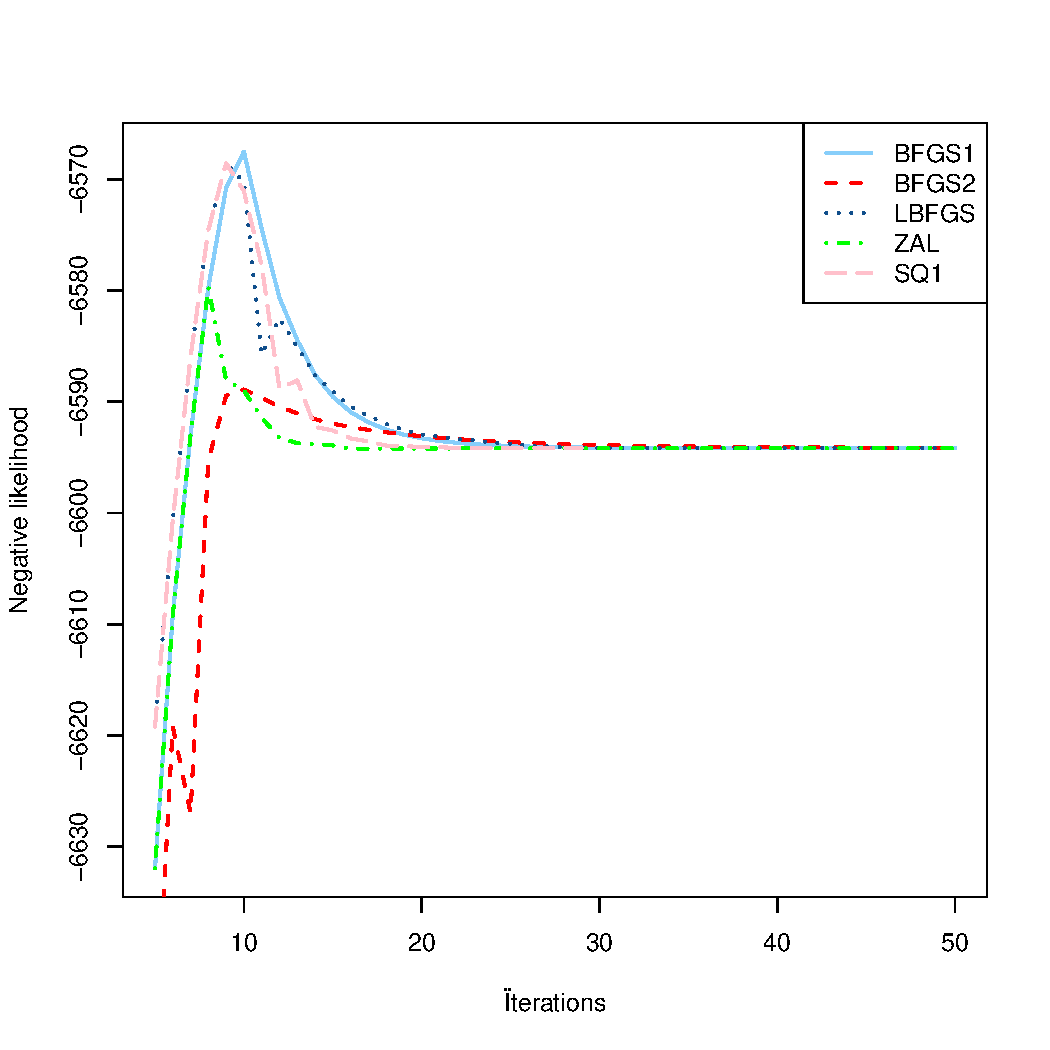
\includegraphics[width = .6\textwidth]{plots/multiT-running.pdf}
    \caption{Multivariate t-distribution. Running plot of negative likelihood vs number of iterations \jx{need to fix plot so that likelihood is only decreasing with iteration?}}
    \label{fig:multiT-running}
\end{figure}

 The PX-EM method of \cite{meng1997algorithm} differs only in update of $\Sigma$ by replacing the denominator N by $\sum_{i}w_i$. We will use a randomly generated data for $\nu = 1$ (multivariate Cauchy distribution) with parameters $\mu = 0$ and $\Sigma = V$ where V is a random symmetrical randomly generated matrix. We will also use $p = 10$ which accounts for 65 parameters (10 for $\mu$ and 55 for $\Sigma$). We report the results for 100 simulations with randomly generated data and use the starting values suggested by \cite{meng1997algorithm}.
 
 \begin{align*}
     \mu_0 &=  \dfrac{1}{N}\sum_{i=1}^{N}y_i\\
     \Sigma_0 &= \dfrac{1}{N}\sum_{i=1}^{N}(y_i - \overline{y})(y_i - \overline{y})^T
 \end{align*}
 

\subsubsection{Landweber's method for quadratic minimization}

\jx{If we do derive some theory and we assume conditions such as Lipschitz, then we may move this example up first and say that it is meant to confirm the theory in practice, i.e. we observe superlinear rate compared to the unaccelerated algorithm}.

In this example, we deal with a simple problem of minimizing a quadratic function $f(\theta)$ using an MM iterative scheme. Landweber's method identifies a maximizing function for the quadratic equation using the Lipchitz property of gradient of $f(\theta)$. Suppose the quadratic function is of the form 
\[
f(\theta) = \dfrac{1}{2}\theta^T A \theta + b^T \theta
\]
where $A$ is a $p \times p$ positive definite matrix. The exact solution is available by solving the linear equation $A\theta = -b$. This operation has an order of complexity of $\mathcal{O}(p^3)$. Therefore, we will explore the iterative scheme explained in \cite{lange2016mm}. We know that $\nabla f(\theta) = A \theta + b$. Therefore, we can write the gradient inequality
%
\[
\|\nabla f(\theta) - \nabla f(\Phi)\| = \|A(\theta - \Phi)\| \leq \|A\|\|\theta - \Phi\|
\]
%
As a consequence, spectral norm of A is the Lipchitz constant for $\nabla f(\theta)$. Consider $L > \|A\|$ to be the Lipschitz constant for $\nabla f(\theta)$, then Lendweber's method gives the following maximization for $f(\theta)$
%
\begin{align*}
    f(x) \leq f(y) + df(y) (x-y) + \dfrac{L}{2}\|x-y\|^2
\end{align*}
Minimizing the above maximizer gives the following update formula
\[
\theta_{n+1} = \theta_n - \dfrac{1}{L}\nabla f(\theta_n) = \theta_n - \dfrac{1}{L}(A\theta_n + b)
\]
We consider a high dimensional problem with $p = 1000$. The starting value for all the replications are 


\begin{table}[!h]
\centering
\begin{tabular}{c c c c c} 
 \hline
 Algorithm & Fevals  & Time & Likelihood\\ [0.5ex] 
 \hline
 MM & 2290 & 0.529 & -0.6427\\
 BFGS1 & 106 & 0.009 & -0.6427\\
 BFGS2 & 35 & 0.004 & -0.6427\\
 LBFGS & 25 & 0.001 & -0.6427 \\
 SqS1 & 60 & 0.002 & -0.6427  \\
 SqS2 & 210 & 0.006 & -0.6427\\
 SqS3 & 72 & 0.001 & -0.6427  \\
 ZAL & 231 & 0.20 & -0.6427  \\[1ex] 
 \hline
\end{tabular}
\caption{Quadratic Minimization. Minimizing the quadratic function $f(\theta) = \theta^T A \theta/2 + b^T \theta$. The number of parameters is $5$ and the stopping criterion is $\epsilon = 10^{-7}$. The starting value is generated randomly.}
\label{tab:quadratic}
\end{table}

\begin{figure}[!htbp]
    \centering
    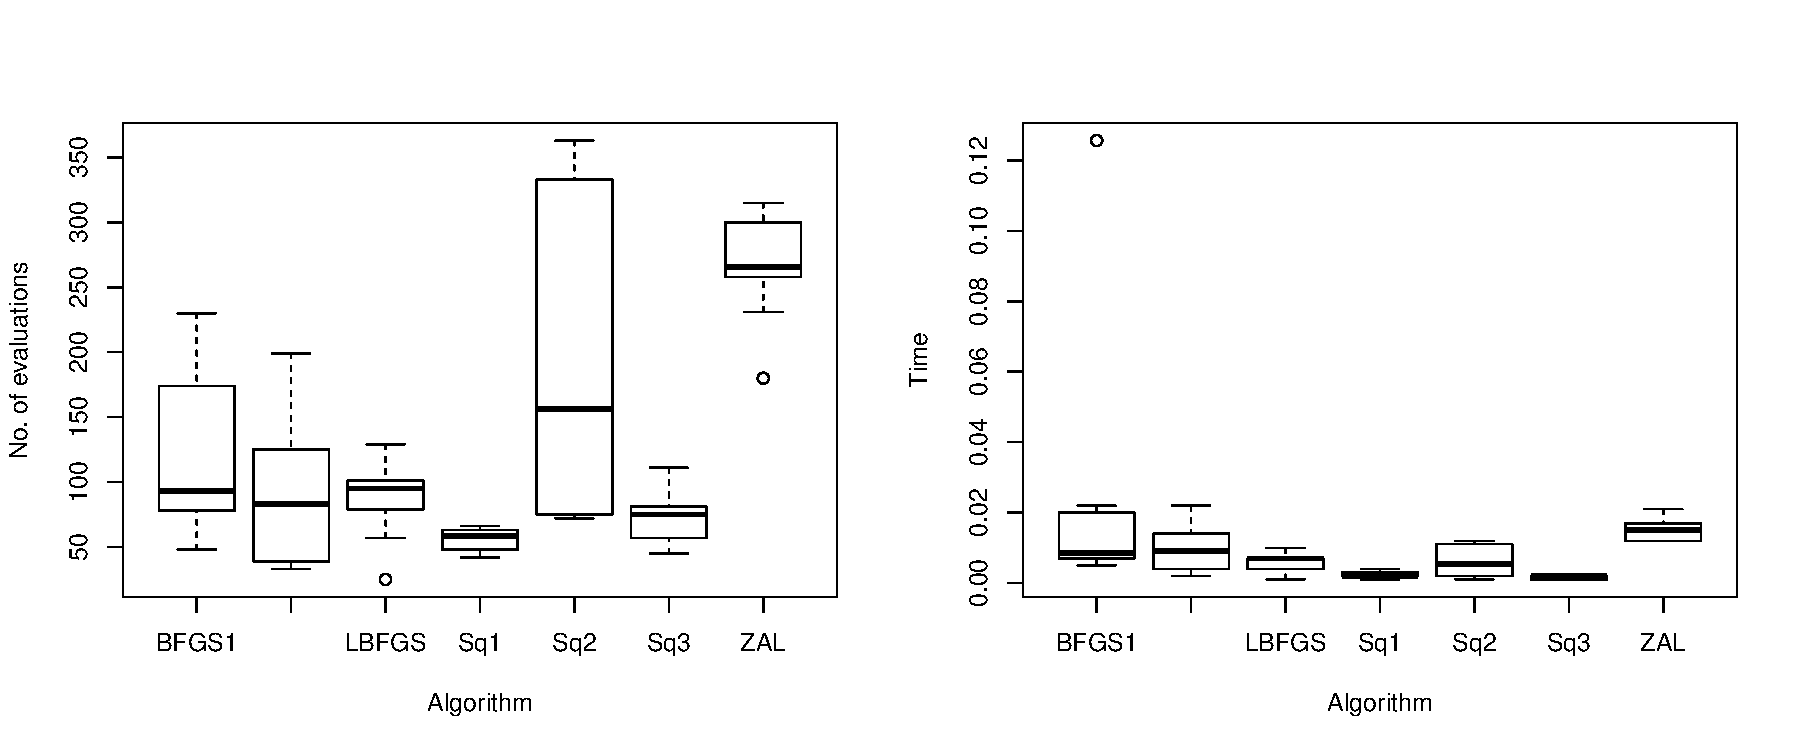
\includegraphics[width = \textwidth]{plots/quad-boxplot_sd1e3.pdf}
    \caption{Quadratic minimization. Boxplots for objective value, number of updates, and time taken for all the compared algorithms.}
    \label{fig:quad_boxplot}
\end{figure}

% \subsection{Examples} \label{subsec:L-BFGSex}


% The prime motivation for the following experiments is to compare the performance of limited memory BFGS, standard BFGS, SQUAREM and ZAL for high dimensional cases. The limited memory method is implemented by storing a certain $m$ number of n-dimensional vector pairs $(u_i, v_i)$ instead of storing the entire $n \times n$ Hessian matrix $H_i$. For our experiments, we will use $m=10$. We stop at iteration $t$ whenever $\|F(x_t) - x_t\|^2 \leq \epsilon$ where $\epsilon = 10^{-7}$. Two examples from section \ref{subsec:BFGSex} have been modified to a high dimensional case and compared to other methods. These are a) Multivariate t-distribution and b) generalized Eigenvalues examples.

% \subsubsection{Multivariate t-distribution}

% Like example \ref{ex:multi.t.distr}, we try to fit a Cauchy model ($\nu = 1$) to data generated from multivariate t-distribution. There is no closed form MLE solution but using the data augmentation technique, one can find the MLE using weighted least squares method. We will accelerate the EM algorithm described by \cite{varadhan2008simple} for a $p = 50$ which accounts for 1325 parameters (50 for $\mu$ and 1275 for the symmetric matrix $\Sigma$). The data is generated from using $\mu = \textbf{0}$ and a randomly generated covariance matrix.\\
% \\
% It can been in Table \ref{tab:t-dist2} that L-BFGS performs way better than BFGS based quasi Newton method with respect to running time. This can be attributed to high time and memory requirements associated with BFGS method in storing and performing matrix multiplication for $1325 \times 1325$ Hessian matrices.
% \begin{table}[h!]
% \centering
% \begin{tabular}{c c c c c} 
%  \hline
%  Algorithm & Fevals & Levals & Time & Likelihood\\ [0.5ex] 
%  \hline
%  EM & 1007 & 1007 & 3.7911  & -19322.47\\ 
%  PX-EM & 50 & 50 & 0.2263 & -19322.47 \\
%  ZAL & 1046 & 1046 & 7.3111 & -19322.47 \\
%  SqS1 & 114 & 46 & 0.6382 &  -19322.47 \\
%  SqS2 & 102 & 44 & 0.5794 & -19322.47 \\
%  SqS3 & 87 & 37 & 0.4627 & -19322.47\\
%  BFGS & 141 & 141 &  110.892 & -19322.47\\
%  L-BFGS & 114 & 46 & 0.5625 & -19322.47 \\
%  JJ-QN1 & 66 & 0 & 1.6766 & -19322.47 \\[1ex] 
%  \hline
% \end{tabular}
% \caption{Parameter estimation of a 1325-dimensional multivariate t-distribution, with 1 degree of freedom with $\mu = 0$, and a randomly generated covariance matrix.}
% \label{tab:t-dist2}
% \end{table}

\bibliographystyle{apalike}
\bibliography{ref}
\end{document}